\chapter{Arhitektura i dizajn sustava}
		
		\textbf{\textit{dio 1. revizije}}\\

		\textit{ Potrebno je opisati stil arhitekture te identificirati: podsustave, preslikavanje na radnu platformu, spremišta podataka, mrežne protokole, globalni upravljački tok i sklopovsko-programske zahtjeve. Po točkama razraditi i popratiti odgovarajućim skicama:}
	\begin{itemize}
		\item 	\textit{izbor arhitekture temeljem principa oblikovanja pokazanih na predavanjima (objasniti zašto ste baš odabrali takvu arhitekturu)}
		\item 	\textit{organizaciju sustava s najviše razine apstrakcije (npr. klijent-poslužitelj, baza podataka, datotečni sustav, grafičko sučelje)}
		\item 	\textit{organizaciju aplikacije (npr. slojevi frontend i backend, MVC arhitektura) }		
	\end{itemize}

	
		

		

				
		\section{Baza podataka}
		
		Aplikacija koristi SQL relacijsku bazu podataka. Ona se sastoji od relacija (tablica) koje se sastoje od atributa. Razlog uporabe relacijske baze podataka je olakšavanje modeliranja entiteta i događaja iz stvarnog svijeta. Baza podataka ove aplikacije sastoji se od sljedećih entiteta:
		
		\begin{packed_item}
			
			\item Korisnik
			\item Kontejner
			\item Komunalna služba
			\item Pretplata
			\item Recenzija
			\item Senzor
			\item Zona
			\item Grad
			\item Država
			
		\end{packed_item}
		
			\subsection{Opis tablica}
				
				\textbf{Korisnik.} Ovaj entitet sadrži informacije o korisniku aplikacije. Uključeni atributi su ID korisnika, ID komunalne službe u kojoj je korisnik zaposlen (ako je zaposlen u komunalnoj službi), korisničko ime, e-mail adresa, informacije je li e-mail adresa potvrđena te lozinka. Ovaj entitet u vezi je \textit{One-to-Many} s entitetom Komunalna služba preko ID-a korisnika te u vezi \textit{Many-to-One} s entitetom Komunalna služba preko ID-a komunalne službe u kojoj je korisnik zaposlen.
				
				\begin{longtabu} to \textwidth {|X[6, l]|X[6, l]|X[20, l]|}
					
					\hline \multicolumn{3}{|c|}{\textbf{Korisnik}}\\[3pt] \hline
					\endfirsthead
					
					\hline \multicolumn{3}{|c|}{\textbf{Korisnik}}\\[3pt] \hline
					\endhead
					
					\hline 
					\endlastfoot
					
					\cellcolor{LightGreen}IDkorisnik & INTEGER & Jedinstveni identifikator korisnika\\ \hline
					\cellcolor{LightBlue}IDsluzba & INTEGER & Jedinstveni identifikator komunalne službe\\ \hline 
					korisnickoIme & VARCHAR & Korisničko ime\\ \hline 
					email & VARCHAR & E-mail adresa korisnika\\ \hline 
					emailPotvrda & BOOLEAN & Stanje potvrđenosti e-mail adrese\\ \hline 
					lozinka & VARCHAR & Hash lozinke\\ \hline 
					
				\end{longtabu}
			
				\textbf{Kontejner.} Ovaj entitet sadrži informacije o kontejneru. Uključeni atributi su ID kontejnera, ID komunalne službe, ID zone u kojoj se kontejner nalazi, adresa kontejnera, geografska dužina te geografska širina kontejnera. Ovaj entitet u vezi je \textit{One-to-Many} s entitetom Pretplata, Recenzija i Senzor preko ID-a kontejnera, \textit{Many-to-One} s entitetom Komunalna služba preko ID-a komunalne službe te u vezi \textit{Many-to-One} s entitetom Zona preko ID-a zone.
				
				\begin{longtabu} to \textwidth {|X[6, l]|X[6, l]|X[20, l]|}
					
					\hline \multicolumn{3}{|c|}{\textbf{Kontejner}}\\[3pt] \hline
					\endfirsthead
					
					\hline \multicolumn{3}{|c|}{\textbf{Kontejner}}\\[3pt] \hline
					\endhead
					
					\hline 
					\endlastfoot
					
					\cellcolor{LightGreen}IDkontejner & INTEGER & Jedinstveni identifikator kontejnera\\ \hline
					\cellcolor{LightBlue}IDsluzba & INTEGER & Jedinstveni identifikator komunalne službe\\ \hline 
					\cellcolor{LightBlue}IDzona & INTEGER & Jedinstveni identifikator gradske zone\\ \hline 
					adresa & VARCHAR & Adresa kontejnera\\ \hline 
					geoDuzina & NUMERIC & Geografska dužina kontejnera\\ \hline 
					geoSirina & NUMERIC & Geografska širina kontejnera\\ \hline 
					
				\end{longtabu}
			
				\textbf{Komunalna služba.} Ovaj entitet sadrži informacije o komunalnoj službi. Uključeni atributi su ID komunalne službe, ID direktora komunalne službe, ime komunalne službe te opis komunalne službe. Ovaj entitet u vezi je \textit{One-to-Many} s entitetom Korisnik i Kontejner preko ID-a komunalne službe te u vezi \textit{Many-to-One} s entitetom Korisnik preko ID-a direktora komunalne službe.
				
				\begin{longtabu} to \textwidth {|X[6, l]|X[6, l]|X[20, l]|}
					
					\hline \multicolumn{3}{|c|}{\textbf{Komunalna služba}}\\[3pt] \hline
					\endfirsthead
					
					\hline \multicolumn{3}{|c|}{\textbf{Komunalna služba}}\\[3pt] \hline
					\endhead
					
					\hline 
					\endlastfoot
					
					\cellcolor{LightGreen}IDsluzba & INTEGER & Jedinstveni identifikator komunalne službe\\ \hline
					\cellcolor{LightBlue}IDdirektor & INTEGER & Jedinstveni identifikator direktora komunalne službe\\ \hline 
					imeSluzba & VARCHAR & Ime komunalne službe\\ \hline 
					opisSluzba & VARCHAR & Opis komunalne službe\\ \hline
					
				\end{longtabu}
			
				\textbf{Pretplata.} Ovaj entitet sadrži informacije o korisničkim pretplatama na kontejnere. Uključeni atributi su ID korisnika i ID kontejnera. Ovaj entitet u vezi je \textit{Many-to-One} s entitetom Korisnik preko ID-a korisnika te u vezi \textit{Many-to-One} s entitetom Kontejner preko ID-a kontejnera.
				
				\begin{longtabu} to \textwidth {|X[6, l]|X[6, l]|X[20, l]|}
					
					\hline \multicolumn{3}{|c|}{\textbf{Pretplata}}\\[3pt] \hline
					\endfirsthead
					
					\hline \multicolumn{3}{|c|}{\textbf{Pretplata}}\\[3pt] \hline
					\endhead
					
					\hline 
					\endlastfoot
					
					\cellcolor{LightGreen}IDkorisnik & INTEGER & Jedinstveni identifikator komunalne službe\\ \hline
					\cellcolor{LightGreen}IDkontejner & INTEGER & Jedinstveni identifikator direktora komunalne službe\\ \hline 
					
				\end{longtabu}
			
				\textbf{Recenzija.} Ovaj entitet sadrži informacije o recenzijama kontejnera. Uključeni atributi su ID recenzije, ID korisnika, ID kontejnera, ocjena punoće, ocjena urednosti, komentar, slika te vrijeme objave recenzije. Ovaj entitet u vezi je \textit{Many-to-One} s entitetom Korisnik preko ID-a korisnika te u vezi \textit{Many-to-One} s entitetom Kontejner preko ID-a kontejnera.
				
				\begin{longtabu} to \textwidth {|X[6, l]|X[6, l]|X[20, l]|}
					
					\hline \multicolumn{3}{|c|}{\textbf{Recenzija}}\\[3pt] \hline
					\endfirsthead
					
					\hline \multicolumn{3}{|c|}{\textbf{Recenzija}}\\[3pt] \hline
					\endhead
					
					\hline 
					\endlastfoot
					
					\cellcolor{LightGreen}IDrecenzija & INTEGER & Jedinstveni identifikator recenzije\\ \hline
					\cellcolor{LightBlue}IDkorisnik & INTEGER & Jedinstveni identifikator korisnika\\ \hline 
					\cellcolor{LightBlue}IDkontejner & INTEGER & Jedinstveni identifikator kontejnera\\ \hline 
					ocjenaPunoce & INTEGER & Ocjena punoće kontejnera\\ \hline
					ocjenaUrednosti & INTEGER & Ocjena urednosti kontejnera\\ \hline
					komentar & VARCHAR & Komentar na stanje kontejnera u trenutku objavljivanja recenzije\\ \hline
					slika & LONGBLOB & Slika kontejnera u trenutku objavljivanja recenzije\\ \hline
					vrijemeObjave & TIMESTAMP & Vrijeme u trenutku objavljivanja recenzije\\ \hline
					
				\end{longtabu}
			
				\textbf{Senzor.} Ovaj entitet sadrži informacije o senzoru. Uključeni atributi su ID senzora, ID kontejnera te token. Ovaj entitet u vezi je \textit{Many-to-One} s entitetom Kontejner preko ID-a kontejnera.
				
				\begin{longtabu} to \textwidth {|X[6, l]|X[6, l]|X[20, l]|}
					
					\hline \multicolumn{3}{|c|}{\textbf{Senzor}}\\[3pt] \hline
					\endfirsthead
					
					\hline \multicolumn{3}{|c|}{\textbf{Senzor}}\\[3pt] \hline
					\endhead
					
					\hline 
					\endlastfoot
					
					\cellcolor{LightGreen}IDsenzor & INTEGER & Jedinstveni identifikator senzora\\ \hline
					\cellcolor{LightBlue}IDkontejner & INTEGER & Jedinstveni identifikator kontejnera\\ \hline 
					token & VARCHAR & Token senzora\\ \hline
					
				\end{longtabu}
			
				\textbf{Zona.} Ovaj entitet sadrži informacije o gradskoj zoni u kojoj je smješten kontejner. Uključeni atributi su ID zone, ID grada te ime zone. Ovaj entitet u vezi je \textit{One-to-Many} s entitetom Kontejner preko ID-a zone te u vezi \textit{Many-to-One} s entitetom Grad preko ID-a grada.
				
				\begin{longtabu} to \textwidth {|X[6, l]|X[6, l]|X[20, l]|}
					
					\hline \multicolumn{3}{|c|}{\textbf{Zona}}\\[3pt] \hline
					\endfirsthead
					
					\hline \multicolumn{3}{|c|}{\textbf{Zona}}\\[3pt] \hline
					\endhead
					
					\hline 
					\endlastfoot
					
					\cellcolor{LightGreen}IDzona & INTEGER & Jedinstveni identifikator gradske zone\\ \hline
					\cellcolor{LightBlue}IDgrad & INTEGER & Jedinstveni identifikator grada\\ \hline 
					imeZona & VARCHAR & Ime zone\\ \hline
					
				\end{longtabu}
			
				\textbf{Grad.} Ovaj entitet sadrži informacije o gradu u kojoj je smješten kontejner. Uključeni atributi su ID grada, ID države te ime grada. Ovaj entitet u vezi je \textit{One-to-Many} s entitetom Zona preko ID-a grada te u vezi \textit{Many-to-One} s entitetom Država preko ID-a države.
				
				\begin{longtabu} to \textwidth {|X[6, l]|X[6, l]|X[20, l]|}
					
					\hline \multicolumn{3}{|c|}{\textbf{Grad}}\\[3pt] \hline
					\endfirsthead
					
					\hline \multicolumn{3}{|c|}{\textbf{Grad}}\\[3pt] \hline
					\endhead
					
					\hline 
					\endlastfoot
					
					\cellcolor{LightGreen}IDgrad & INTEGER & Jedinstveni identifikator grada\\ \hline
					\cellcolor{LightBlue}IDdrzava & INTEGER & Jedinstveni identifikator države\\ \hline 
					imeGrad & VARCHAR & Ime grada\\ \hline
					
				\end{longtabu}
			
				\textbf{Država.} Ovaj entitet sadrži informacije o državi u kojoj je smješten kontejner. Uključeni atributi su ID države te ime države. Ovaj entitet u vezi je \textit{One-to-Many} s entitetom Grad preko ID-a države.
				
				\begin{longtabu} to \textwidth {|X[6, l]|X[6, l]|X[20, l]|}
					
					\hline \multicolumn{3}{|c|}{\textbf{Država}}\\[3pt] \hline
					\endfirsthead
					
					\hline \multicolumn{3}{|c|}{\textbf{Države}}\\[3pt] \hline
					\endhead
					
					\hline 
					\endlastfoot
					
					\cellcolor{LightGreen}IDdrzava & INTEGER & Jedinstveni identifikator države\\ \hline
					imeDrzava & VARCHAR & Ime države\\ \hline
					
				\end{longtabu}
			
			
			
			
			\subsection{Dijagram baze podataka}
				\begin{figure}[H]
					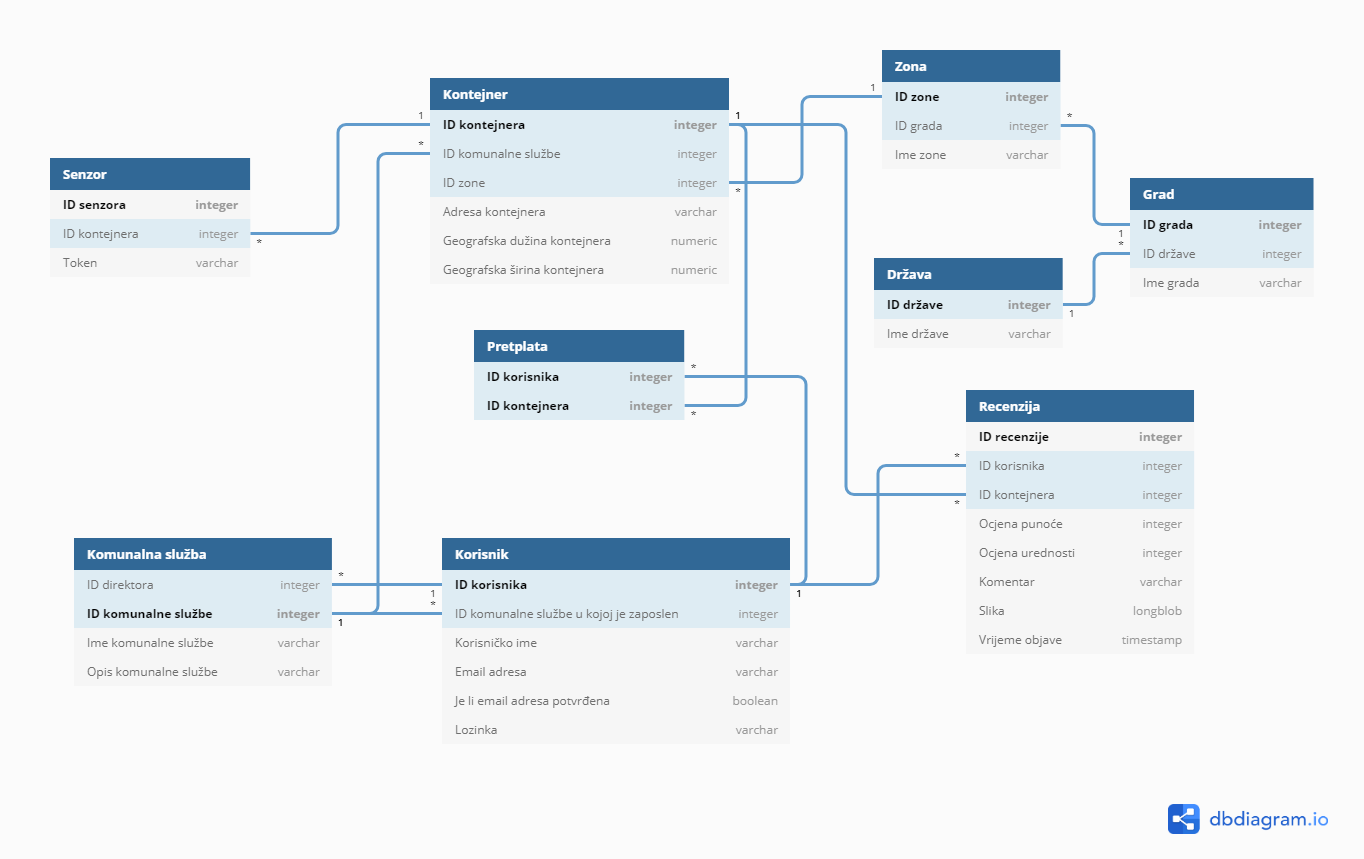
\includegraphics[width=1.0\linewidth]{slike/dijagramBaze.png}
					\centering
					\caption{Dijagram baze podataka}
					\label{fig:promjene}
				\end{figure}
			
			Dijagram baze podataka je izrađen alatom \href{https://dbdiagram.io}{dbdiagram.io}. Svjetlo plavo su označeni strani ključevi, a primarni ključevi su podebljani. 
			
			\eject
			
			
		\section{Dijagram razreda}
		
			\textit{Potrebno je priložiti dijagram razreda s pripadajućim opisom. Zbog preglednosti je moguće dijagram razlomiti na više njih, ali moraju biti grupirani prema sličnim razinama apstrakcije i srodnim funkcionalnostima.}\\
			
			\textbf{\textit{dio 1. revizije}}\\
			
			\textit{Prilikom prve predaje projekta, potrebno je priložiti potpuno razrađen dijagram razreda vezan uz \textbf{generičku funkcionalnost} sustava. Ostale funkcionalnosti trebaju biti idejno razrađene u dijagramu sa sljedećim komponentama: nazivi razreda, nazivi metoda i vrste pristupa metodama (npr. javni, zaštićeni), nazivi atributa razreda, veze i odnosi između razreda.}\\
			
			\textbf{\textit{dio 2. revizije}}\\			
			
			\textit{Prilikom druge predaje projekta dijagram razreda i opisi moraju odgovarati stvarnom stanju implementacije}
			
			
			
			\eject
		
		\section{Dijagram stanja}
			
			
			\textbf{\textit{dio 2. revizije}}\\
			
			\textit{Potrebno je priložiti dijagram stanja i opisati ga. Dovoljan je jedan dijagram stanja koji prikazuje \textbf{značajan dio funkcionalnosti} sustava. Na primjer, stanja korisničkog sučelja i tijek korištenja neke ključne funkcionalnosti jesu značajan dio sustava, a registracija i prijava nisu. }
			
			
			\eject 
		
		\section{Dijagram aktivnosti}
			
			\textbf{\textit{dio 2. revizije}}\\
			
			 \textit{Potrebno je priložiti dijagram aktivnosti s pripadajućim opisom. Dijagram aktivnosti treba prikazivati značajan dio sustava.}
			
			\eject
		\section{Dijagram komponenti}
		
			\textbf{\textit{dio 2. revizije}}\\
		
			 \textit{Potrebno je priložiti dijagram komponenti s pripadajućim opisom. Dijagram komponenti treba prikazivati strukturu cijele aplikacije.}